\documentclass[letterpaper,final,12pt,reqno]{amsart}

\usepackage[total={6.3in,9.2in},top=1.1in,left=1.1in]{geometry}

\usepackage{times,bm,empheq,fancyvrb,graphicx}
\usepackage[dvipsnames]{xcolor}
\usepackage{tikz}

% hyperref should be the last package we load
\usepackage[pdftex,
colorlinks=true,
plainpages=false, % only if colorlinks=true
linkcolor=blue,   % ...
citecolor=Red,    % ...
urlcolor=black    % ...
]{hyperref}

\renewcommand{\baselinestretch}{1.05}

\newtheorem{lemma}{Lemma}

\newcommand{\Matlab}{\textsc{Matlab}\xspace}
\newcommand{\eps}{\epsilon}
\newcommand{\RR}{\mathbb{R}}

\newcommand{\grad}{\nabla}
\newcommand{\Div}{\nabla\cdot}
\newcommand{\trace}{\operatorname{tr}}

\newcommand{\hbn}{\hat{\mathbf{n}}}

\newcommand{\bg}{\mathbf{g}}
\newcommand{\bn}{\mathbf{n}}
\newcommand{\bu}{\mathbf{u}}
\newcommand{\bv}{\mathbf{v}}
\newcommand{\bx}{\mathbf{x}}

\newcommand{\bV}{\mathbf{V}}
\newcommand{\bX}{\mathbf{X}}

\newcommand{\bxi}{\bm{\xi}}

\newcommand{\bzero}{\bm{0}}

\newcommand{\Href}{H_{\text{ref}}}


\begin{document}
\title[Performance of evolving-geometry simulations using Stokes dynamics]{Performance of evolving-geometry glacier and ice sheet simulations using Stokes dynamics}

\author{Ed Bueler}

\maketitle

\thispagestyle{empty}
\bigskip

\section{Introduction} \label{sec:intro}

The most important questions in glaciology concern how the climate around a glacier determines its geometry, both through changes in the climate along the ice surface and, less directly, through internal flow dynamics.  Relationships between surface mass inputs and the geometry of the ice mass are important because they affect sea level, deformations of the Earth's crust, and fresh water supplies, among other concerns.  Because of such concerns, evolving-geometry simulations are widely used by scientists to understand the size and extent of glaciers and ice sheets.

A variety of methodologies for such numerical simulations are seen in practice, with most of the well-established schemes involving shallowness approximations of the continuum equations \cite[for example]{Hoffmanetal2018,Lipscombetal2019,Winkelmannetal2011}.  Furthermore, most methods use explicit or semi-implicit time-stepping \cite{HindmarshPayne1996,Hoffmanetal2018,Lipscombetal2019,Winkelmannetal2011}, with small stability-imposed time steps at high spatial resolution, though fully-implicit exceptions exist \cite{Brinkerhoffetal2017,Bueler2016}.  The performance properties of current numerical models limit either the physical modeling authenticity (due to shallowness and other approximations) or the spatial resolution (due to time-stepping and solver performance limitations).  In particular, the quality of ensemble simulations, regarding both the number of ensemble members and the quality of the individual simulations, is directly limited by numerical model performance.

This paper\footnote{version: \today.  Co-author thoughts: L.~Mitchell because of \texttt{SemiCoarsened...()} etc.~ code (actual).  C.~Khrulev because of implementation and analysis help (prospect).  R.~Sayag because of validation experiment (prospect).  M.~Knepley because of performance help and analysis (prospect).} addresses an important, but also restricted, class of numerical glacier and ice sheet models, based on conservation of momentum and mass and without shallowness assumptions.  For conservation of momentum we use the standard shear-thinning (Glen) power-law Stokes model.  Noting that ``mass conservation'' properly refers both to fluid incompressibility and to conservation at the ice surface, we solve both the divergence-free equation for bulk ice and the surface kinematical equation (or kinematic boundary condition \cite{GreveBlatter2009}) with the surface mass balance is an input.  We model three-dimensional (3D) grounded glaciers and ice sheets for which there is a well-defined ice thickness; overhanging ice is not modeled.  The ice thickness is defined at all map-plane points but it is zero in those locations where the (coupled and solved) surface balance and ice flow do not determine the presence of glacier ice, and the solution process also determines the location of the free boundary at the ice margin \cite{SchoofHewitt2013} (Figure \ref{fig:cartoon}).

\begin{figure}[h]
\begin{center}
\includegraphics[width=0.7\textwidth]{figs/cartoon.pdf}
\end{center}
\caption{We consider 3D models of grounded glaciers and ice sheets which are based on Glen-Stokes ice flow, an evolving free surface, and a free boundary.}
\label{fig:cartoon}
\end{figure}

We do not, however, consider the conservation of energy, and neither thermomechanical coupling nor basal melt are included in our model.  A further restriction is that our ice sticks to the bed (no slip), and we do not consider floating ice.  Finally we only consider cases where the bed elevations are relatively-smooth.  These restrictions are all removable by well-known modeling mechanisms \cite[for example]{Aschwandenetal2012,Winkelmannetal2011}, but how these components affect model performance is a topic for further research.

To discretize the continuum equations we apply the finite element (FE) method \cite{Elmanetal2014} by using the Firedrake library \cite{Rathgeberetal2016} in Python.\footnote{These Python programs are open-source at \href{https://github.com/bueler/stokes-implicit}{\texttt{github.com/bueler/stokes-implicit}}.  FIXME: MAKE REPO PUBLIC.}  We use meshes which are unstructured in the map-plane but which are extruded \cite{Gibsonetal2019} in the vertical direction, and we apply semicoarsening in the vertical direction \cite{Tuminaroetal2016}.  As discussed below, mixed elements for velocity, pressure, and vertical ice strain are used, with stable and aspect-ratio robust choices for the velocity-pressure (i.e.~Stokes) block \cite{Elmanetal2014}.  Solutions of the resulting nonlinear discrete equations apply multigrid-preconditioned Newton-Krylov methods \cite{Bueler2021} via PETSc \cite{Balayetal2020}, and all computations are parallelized.

The model performance metric introduced here is a natural one for glacier modeling.  Namely, we measure the run time of our coupled Glen-Stokes simulations relative to the well-understood computation of ice velocity in the shallow ice approximation (SIA) \cite{Fowler1997} on the same mesh.  That is, we define a glacier model ``work unit'' as the time needed for a diagnostic computation of the SIA velocity solution.

FIXME compare the literature of existing glacier Stokes solvers; nonevolving surface \cite{IsaacStadlerGhattas2015,Lengetal2013,Lengetal2014a,Tuminaroetal2016,Zwingeretal2007} (CHECK); explicitly evolving surface \cite{Gudmundsson1999,HelanowAhlkrona2018,Jouvetetal2008,Larouretal2012,
Lengetal2012,Lengetal2014b,LeysingerGudmundsson2004,PralongFunk2004,Seddiketal2012} (CHECK)

The primary purpose of this paper is to understand the performance characteristics of numerical simulations using fully-implicit time-stepping with evolving-surface Glen-Stokes models.  That is, at each time step the stress balance, incompressibility, and surface kinematical equations are solved simultaneously to within a tolerance on the coupled residual.  (Only the interaction between ice surface elevation and the evaluation of surface mass balance is split in time.)  Time steps of order one year are targeted.  To evaluate our approach we validate the model based on results of laboratory experiments, we compare the performance of the model with shallow models, we demonstrate solver optimality and scalability, and we show a solution for the Greenland ice sheet.


\section{Equations for ice flow in glaciers} \label{sec:strongform}

The standard model for the flow of glaciers uses Stokes equations based upon Glen's shear-thinning flow law for ice \cite{GreveBlatter2009,JouvetRappaz2011,SchoofHewitt2013}.  We will apply this model on time-dependent $d=2$ or $d=3$ dimensional domains using time $t>0$ and spatial variables $\bx=(x,y,z)$, with $z$ vertical.  (Coordinates are denoted $(x,z)$ in 2D.)  The evolving domain $\Omega^t \subset \RR^d$ will have a piecewise smooth boundary, so that we may apply the boundary conditions, but it is otherwise general.

Allowing any Glen exponent $n\ge 1$, the strong-form model equations are:
\begin{align}
- \nabla \cdot \tau + \nabla p &= \rho \bg &&\text{\emph{stress balance}} \label{forcebalance} \\
\nabla \cdot \bu &= 0 &&\text{\emph{incompressibility}} \label{incompressible} \\
\tau &= B_n |D\bu|^{(1/n) - 1} D\bu  &&\text{\emph{flow law}} \label{viscflowlaw}
\end{align}
The solution fields are velocity $\bu$, pressure $p$, and deviatoric stress tensor $\tau$.  For simplicity we take the ice density $\rho$ and the acceleration of gravity $\bg=\left<0,0,-g\right>$, with $g>0$, to be constant.

Regarding tensors and their notation, the full (Cauchy) stress tensor $\sigma$ decomposes into the deviatoric part $\tau$ minus the pressure, i.e.~$\sigma = \tau - p\,I$, so equation \eqref{forcebalance} simply says $-\Div \sigma = \rho \bg$.  The strain rate tensor $D\bu$ is the symmetric part of $\grad \bu$, i.e.~$(D\bu)_{ij} = \frac{1}{2} \left(\grad\bu + \grad\bu^\top\right)$.  Because $D\bu$ is symmetric, and because it has trace zero by equation \eqref{incompressible}, i.e.~$\trace(D\bu)=\nabla \cdot \bu = 0$, from equation \eqref{viscflowlaw} it follows that $\tau$ is also symmetric with trace zero.  The tensor norm in \eqref{viscflowlaw} satisfies $|D\bu|^2 = \frac{1}{2} \trace\left((D\bu)^2\right) = \frac{1}{2} (D\bu)_{ij} (D\bu)_{ij}$.  Note $B_n$ is the $n$-dependent ice hardness in units $\text{Pa}\,\text{s}^{1/n}$, sometimes written $B_n = (A_n)^{-1/n}$ in terms of the softness $A_n$.

For the linear Stokes equations \cite{Elmanetal2014}, i.e.~the $n=1$ case, one would traditionally write the flow law \eqref{viscflowlaw} as $\tau = 2\nu D\bu$, and in that case the viscosity would be $\nu = (1/2) B_1$.  For realistic powers $n>1$, namely shear-thinning ice, one defines an ``effective viscosity'' in equation \eqref{viscflowlaw} which involves a negative power of the strain rate magnitudes $|D\bu|$.  This effective viscosity would be singular in the limit of small strain rates, and so, motivated by the expected finite viscosity of glacier ice \cite{GreveBlatter2009}, and noting the equations using such a regularization are well-posed \cite{JouvetRappaz2011}, we define the regularized effective viscosity
\begin{equation}
\nu_\eps(|D\bu|) = (1/2) B_n \left(|D\bu|^2 + \eps\, D_0^2\right)^{(r-2)/2} \label{regeffvisc}
\end{equation}
where $\eps = 10^{-4}$ and $r=(1/n)+1$.  The constant $D_0$ defines a strain-rate scale for glacier flow; the value $D_0 = 2 a^{-1}$ used here corresponds to a velocity difference of 1000 meters per year in a distance of 500 meters.

Using \eqref{viscflowlaw}, as modified by \eqref{regeffvisc}, we eliminate $\tau$ from equation \eqref{forcebalance}, thereby rewriting the system in terms of velocity and pressure derivatives only:
\begin{align}
- \nabla \cdot \left(2 \nu_\eps(|D\bu|)\, D\bu\right) + \nabla p &= \rho \mathbf{g} \label{stokes} \\
\Div \bu &= 0 \label{incompagain}
\end{align}
This system is our Glen-Stokes model for bulk ice motion.  A solution is a velocity-pressure pair $(\bu,p)$, from which one may derive strain rates $D\bu$ and stresses $\tau$ and/or $\sigma = \tau - p\,I$.

Glacier-suitable dynamic boundary conditions will be used, with an emphasis on isolated, grounded glaciers.  In such cases the ice flow extends in the horizontal direction until a free boundary at the glacier margin is reached.  (In real glaciers grounded margins may occur as fracture-generated cliffs, but such non-fluid processes are not modeled here.)  As noted in the Introduction, we assume that the ice thickness is well-defined and thus that the top and bottom boundaries of $\Omega^t$ can, at each time, be identified.  On the top surface we set a condition of zero applied stress,
\begin{align}
\left(2 \nu_\eps(|D\bu|) D\bu - pI\right) \bn &= \bzero  &&\text{\emph{top}: } \overline{\partial} \Omega^t \label{topbc} \\
\intertext{where $\bn$ is normal to the surface.  On the base we require no slip:}
\bu &= \bzero  &&\text{\emph{base}: } \underline{\partial} \Omega^t \label{basebc}
\end{align}

Optionally, to allow simulation of a certain laboratory experiment \cite{SayagWorster2013} (below), we also allow inflow.  Here a prescribed velocity is applied, $\bu = \bu_{\text{in}}$ on an inflow boundary $\partial_{\text{in}} \Omega^t$, subject to $\bu_{\text{in}}\cdot \bn \le 0$ where $\bn$ is an outward normal.

Assuming the well-posedness of the above model \eqref{stokes}--\eqref{basebc}, as is proven by \cite{JouvetRappaz2011}, if the ice geometry $\Omega^t$ is known then the solution is a unique pair $(\bu,p)$.  Note that the slowness of the fluid, i.e.~zero Reynolds number, implies that the given boundary stresses and body forces determine velocity and pressure fields without any ``memory'' of prior states or influence from inertia, as would arise in the Navier-Stokes equations \cite{Fowler1997}.

The SIA, a widely-used simplified model for the flow of grounded, non-sliding ice \cite{SchoofHewitt2013}, is used in this paper for comparison purposes.  It is derived by a small-parameter argument which we recall now by following Chapter 18 of \cite{Fowler1997}; note similar arguments in other sources e.g.~\cite{GreveBlatter2009}.  Let $[H]$, $[L]$, $[U]$, and $[\tau]$ denote typical thickness, horizontal extent, horizontal velocity, and vertical-plane shear stress values, respectively.  We consider $\eps = [H]/[L]$ as the small parameter; for a mountain glacier we might have $\eps \approx 0.1$ but for the Greenland ice sheet $\eps \in (10^{-3},10^{-2})$ is reasonable.  We scale the kinematic variables $x,y \sim [L]$, $z \sim [H] = \eps [L]$, $u,v \sim [U]$, and $w \sim \eps [U]$.\footnote{Recall this means, for example, that we introduce new ``hatted'' variables via $x=[L]\hat x$, $y=[L]\hat y$, and $z=[H] \hat z$.  The equations are rewritten in the new variables and then the hats are removed.}  We suppose the stress components $\tau_{xz},\tau_{yz}$ scale with $[\tau]$ and components $\tau_{xx},\tau_{yy},\tau_{xy}$ with $\eps[\tau]$.   The pressure perturbation from the hydrostatic condition, namely $p-\rho g (h - z)$, is scaled with $\eps [\tau]$ also; this means that $p-\rho g (h - z)=\eps[\tau]\hat{\delta p}$.  With these scalings, plus certain additional relationships among the scale factors \cite[Chapter 18]{Fowler1997}, equations \eqref{forcebalance} yield
    $$\frac{\partial\tau_{xz}}{\partial z} + O(\eps^2) = \frac{\partial h}{\partial x}, \qquad \frac{\partial\tau_{yz}}{\partial z} + O(\eps^2) = \frac{\partial h}{\partial y}.$$
The shear stresses are dominated by the $z$ derivatives of the horizontal velocity, that is,
    $$\tau_{xz} = \nu\left(\frac{\partial u}{\partial z} + \eps^2 \frac{\partial w}{\partial z}\right), \qquad \tau_{yz} = \nu\left(\frac{\partial v}{\partial z} + \eps^2 \frac{\partial w}{\partial y}\right).$$
Also, the norm of the deviatoric stress satisfies $|\tau|^2 = \tau_{xz}^2 + \tau_{yz}^2 + O(\eps^2)$ and the stress-free condition at the surface $z=h$ becomes $\tau_{xz} = O(\eps^2)$ and $\tau_{yz} = O(\eps^2)$.  Note that incompressibility \eqref{incompressible} is unaltered by the scaling.

The strong form of the SIA arises from dropping terms of order $O(\eps^2)$ from these equations and returning to the original, unscaled variables.  Let $\bm{\tau}=\left<\tau_{xz},\tau_{yz}\right>$ denote the remaining shear stress components and $\bm{\omega}=\left<\frac{1}{2} \frac{\partial u}{\partial z},\frac{1}{2} \frac{\partial v}{\partial z}\right>$ the corresponding strain rates.  Note that \eqref{viscflowlaw} implies $|\bm{\tau}|=B_n |\bm{\omega}|^{1/n}$, where $|\cdot|$ denotes the ordinary Euclidean norm on $\RR^2$, and thus that $\bm{\omega} = A_n |\bm{\tau}|^{n-1} \bm{\tau}$ where $A_n=(B_n)^{-n}$.  We now have the following equations for the shear stresses and the velocity,
\begin{equation}
\frac{\partial\bm{\tau}}{\partial z} = \rho g \grad h, \qquad \Div \bu = 0, \qquad \bm{\omega} = A_n |\bm{\tau}|^{n-1} \bm{\tau}, \label{siavectorized}
\end{equation}
subject to $\bm{\tau}=0$ at the surface $z=h$ and $\bu=0$ on the base $z=b$.  Note that equations \eqref{siavectorized} essentially use the approximation
    $$D\bu \approx \begin{pmatrix} 0 & 0 & \frac{1}{2} \frac{\partial u}{\partial z} \\  0 & 0 & \frac{1}{2} \frac{\partial v}{\partial z} \\ \frac{1}{2} \frac{\partial u}{\partial z} & \frac{1}{2} \frac{\partial u}{\partial z} & 0 \end{pmatrix}$$
in \eqref{stokes}, and then balance the $z$ derivative of the stresses against the surface gradient.  Note that we need not compute the pressure simultaneously with the velocity.

The SIA stress equations \eqref{siavectorized} can be vertically-integrated to give a formulas for the horizontal velocity.  By a first integral, $\bm{\tau} = - \rho g (h-z) \grad h$, thus
    $$\left<\frac{\partial u}{\partial z},\frac{\partial v}{\partial z}\right> = - 2 A_n (\rho g)^n (h-z)^n |\grad h|^{n-1} \grad h.$$
Integrating again we determine the horizontal velocity at any point within the ice:
\begin{equation}
\left<u,v\right> = - \frac{2 A_n (\rho g)^n}{n+1} \left((h-b)^{n+1} - (h-z)^{n+1}\right) |\grad h|^{n-1} \grad h.  \label{siavelocity}
\end{equation}
The incompressibility equation can then be used to compute the vertical velocity component $w$ by an additional vertical integration of \eqref{siavelocity}, but we have no need for this result.

The result in \eqref{siavelocity} will not be used in this paper as an actual model for ice flow.  Rather it has three ancillary purposes.  First, in combination with the hydrostatic pressure computation $p=\rho g (h-z)$, and the above-mentioned application of incompressibility to find $w$, it provides a fast computation of an initial iterate in a nonlinear Stokes solver.  Second, computing \eqref{siavelocity} on a given mesh defines our ``work unit'' when evaluating Stokes solver performance on that mesh.  Third and finally, when combined with the surface kinematical equation, \eqref{siavelocity} can be used to derive a nonlinear and degenerate diffusion problem for the ice sheet thickness \cite{Fowler1997}.  Appendix A reports an exact similarity solution of this problem, in the flat bed and zero mass-balance case, which we will use as a source of ice sheet initial states in certain numerical experiments.


\section{Ice geometry and its evolution} \label{sec:stronggeometry}

The above equations do not describe how the glacier changes shape or extent.  This process, which is of course coupled to the ice flow velocity, is described by an additional equation which states conservation of mass on the top boundary $\overline{\partial} \Omega^t$.  To present this equation we first assume a larger map-plane computational domain $R\subset \RR^{d-1}$ on which the input surface mass balance and bedrock elevation data of the problem are defined; see Figure \ref{fig:domainnotation}.  The ice-covered area is then a subset of the interior of $R$; that is, we require that ice is not present on, nor does it flow across, the boundary of $R$.

Let $z=b(x,y)$ be the bedrock elevation, assumed continuously-differentiable and time-independent for simplicity, and $z=h(t,x,y)$ be the ice surface elevation; note that both functions are defined for all $(x,y)\in R$.  The surface elevation function, a part of the solution, will be continuous and piecewise differentiable.  The following form for the time-dependent and open ice domain is now assumed:
\begin{equation}
\Omega^t = \left\{\bx\,\big|\,(x,y)\in R \,\text{ and }\, b(x,y) < z < h(t,x,y)\right\}.  \label{Omegat}
\end{equation}
Note that an admissibility requirement \cite{Bueler2016} for $h$, as a part of the model solution, is that at each $t>0$ and $(x,y)\in R$ we have
\begin{equation}
h(t,x,y) \ge b(x,y).  \label{admissibility}
\end{equation}
At any given map-plane location $(x,y)$ the ice may be present (strict inequality in \eqref{admissibility}) or absent (equality) in an evolving, time-dependent manner.  The time-dependent ice-covered map-plane domain, the vertical projection of $\Omega^t$, is denoted $\pi \Omega^t$.

\begin{figure}[h]
\begin{center}
\includegraphics[width=0.7\textwidth]{figs/domainnotation.pdf}
\end{center}
\caption{Notation: The evolving ice domain $\Omega^t$ has projection $\pi \Omega^t$.  Surface mass balance $a$ and bedrock elevation $b$ are defined on all of $R$.}
\label{fig:domainnotation}
\end{figure}

In agreement with almost all ice sheet and glacier modeling literature, equation \eqref{Omegat} states that both the upper and lower surfaces of the ice mass are described by a well-defined functions of map-plane location.  The domain $\Omega^t$ is thus a layer \cite{Bueler2020}, and not general.  In the usual case where $\partial_{\text{in}} \Omega^t=\emptyset$ we assume a disjoint decomposition $\partial \Omega^t = \overline{\partial} \Omega^t \cup \underline{\partial} \Omega^t$ except for a set of measure zero along the margin.  Looking ahead, this layer assumption is compatible with FE numerics based on vertically-extruded meshes which are unstructured mesh in the map plane.

Let $a_\perp(t,x,y,z)$ be the vertical modeled climatic surface mass balance, in (ice-equivalent) units $\text{m}\,\text{s}^{-1}$.  This scalar field must be defined for all locations above the bedrock elevation, i.e.~$(x,y,z) \in R\times[b(x,y),\infty)$.  Denoting the velocity components as $\bu=\left<u,v,w\right>$, the surface kinematical equation \cite{GreveBlatter2009} then applies on the top of the ice,
    $$\frac{\partial h}{\partial t} = a - u \frac{\partial h}{\partial x} - v \frac{\partial h}{\partial y} + w,$$
or, stated more precisely using vector notation,
\begin{equation}
\frac{\partial h}{\partial t} = a + \bu|_{z=h} \cdot \bn \quad \text{ on } \overline{\partial}\Omega^t, \label{surfacekinematical}
\end{equation}
where $\bn = \left<-\frac{\partial h}{\partial x},-\frac{\partial h}{\partial y},1\right>$ is upward and normal to the ice surface.  The surface mass balance $a$ in \eqref{surfacekinematical} is the trace \cite{Evans2010} of the vertical value of the mass balance along the ice surface,
    $$a := a_{\perp}(t,x,y,h(x,y,t)).$$
Modeled melting or freeze-on at the ice base would add a basal kinematic equation \cite[for example]{Aschwandenetal2012}, but for simplicity this is not considered here.

Equation \eqref{surfacekinematical} applies on the ice surface, that is, where ice is present.  However, the equation should be understood as the following pair of statements on the entire computational domain $R$ \cite{Bueler2016,Bueler2020,SchoofHewitt2013}:
\begin{align}
\frac{\partial h}{\partial t} - a|_{z=h} - \bu|_{z=h} \cdot \bn &\ge 0, \label{stronginequality} \\
(h-b) \left(\frac{\partial h}{\partial t} - a|_{z=h} - \bu|_{z=h} \cdot \bn\right) &= 0. \label{strongcomplementarity}
\end{align}
At ice-free locations, where $\frac{\partial h}{\partial t}=0$ and $\bu=\bzero$, \eqref{stronginequality} says that $a \le 0$, that is, the surface mass balance is not positive; physically-speaking, snow melt and runoff exceeds solid precipitation, and also ice is not flowing to that location.  Equation \eqref{strongcomplementarity}, a complementarity principle, says that either there is no ice at the location ($h=b$) or ice is present and equation \eqref{surfacekinematical} applies.  Thus \eqref{stronginequality} and \eqref{strongcomplementarity} together imply \eqref{surfacekinematical} on the ice surface and also that $a\le 0$ at ice-free locations, but they do so without referring to glacier extent, which we regard as part of the solution.

Informally, \eqref{surfacekinematical} describes how the ice surface elevation is updated: the climatically added or removed ice $a\,\Delta t$, plus the component of the ice motion in direction $\bn$, determines the vertical motion of the surface.  Note that the mass balance $a_{\perp}(t,x,y,z)$ is computed using a separate model for the dynamical state of the atmosphere, one which computes snow precipitation, (atmospheric) energy-driven melt at snow/ice surfaces, and liquid water runoff.  How this is done is well beyond our scope, but it is important in moving-margin glacier simulations that $a$ have a well-defined value both at the current ice surface and elsewhere, or at least nearby.  The simulated glacier can only move into new areas, retreat from ice-covered areas, and undergo changes of surface elevation, if the source term at the new (and intermediate) locations is well-defined.

Numerical glacier models often evolve the time-dependent surface $z=h$ by explicit steps, i.e.~$\Delta h \approx \left(a + \bu\cdot \bn\right) \Delta t$ in the simplest forward-Euler case, based upon the current values of $a$, $\bu$, and $\bn$ (i.e.~$\grad h$).  However, we will be solving \eqref{surfacekinematical}, more precisely \eqref{stronginequality} and \eqref{strongcomplementarity}, implicitly and coupled with the Glen-Stokes system \eqref{stokes}--\eqref{basebc}.


\section{Implicit time-stepping and the domain update} \label{sec:implicitstep}

As stated in the Introduction, the main purpose of this paper is to demonstrate an implicit scheme to simultaneously solve the Glen-Stokes equations \eqref{stokes}--\eqref{incompagain} and the surface kinematical equation \eqref{surfacekinematical}.  We will state this scheme using a discrete-time and continuous-space formulation, using first-order backward Euler time-stepping.  A new feature of our scheme is that at each time step this scheme will compute a surrogate for the ice strain over the duration of the time step.  This surrogate, a vertical-only displacement, is defined everywhere within a reference domain.  The displacement will be computed simultaneously with the velocity and pressure, and once found it determines how the domain of ice is updated.

More accurate implicit schemes than backward Euler exist, and one could certainly apply higher-order schemes.  However, the coupled solution is subject to the inequality constraint that the ice thickness is nonnegative, and the resulting free-boundary problem has the character of a time-dependent variational inequality or complementarity problem \cite{Bueler2020}.  The numerical errors associated to determining the free-boundary tend to dominate over time-stepping errors made in well-behaved locations.

The fundamental issue faced by implicit time-stepping schemes for our glacier problem is that the 2D (map-plane) region covered by the ice, and the 3D domain of the ice, will change during the time step.  Either in terms of the (spatial) mesh we will use for numerical simulations, or in terms of the continuum domain on which we solve the coupled PDE problem describing a time step, one can only solve for velocity and pressure in locations where ice exists.  The possiblity of glacier advance and retreat therefore requires us to extend the domain of the solution to cover locations where the glacier currently is (time $t_{n-1}$) and locations where it will be once we have solved the time-step equations ($t_n$).

\begin{figure}[ht]
\begin{center}
\includegraphics[width=0.6\textwidth]{figs/currenttime.pdf}
\vspace{-6mm}

\includegraphics[width=0.6\textwidth]{figs/referencedomain.pdf}
\vspace{-1mm}

\includegraphics[width=0.6\textwidth]{figs/nexttime.pdf}
\end{center}
\caption{The current ice domain $\Omega^{n-1}$ is modified to a reference domain $\Lambda$.  The coupled solution includes a map from $\Lambda$ to the next domain $\Omega^n$ which degenerates where the solution indicates no ice.}
\label{fig:domainupdate}
\end{figure}

We will need a reference glacier thickness $\Href>0$.  This value should have the property that grounded ice of uniform thickness $\Href$ flows very slowly when draped over the bedrock topography, and it should be small compared to observed glacier thicknesses.  For example, values in the range $50 \le \Href \le 500$ m would be appropriate for glaciers ranging from small mountain glaciers to large, cold, and low-angle ice sheets.  Recall that the velocity of Glen $n=3$ ice in a slab-on-slope geometry \cite{GreveBlatter2009} goes as the $4$th power of the ice thickness; $50$ m ice flows $10^4$ times slower than $500$ m ice.

Let $t_{n-1}$ and $t_n$ be consecutive times with step $\Delta t = t_n - t_{n-1} > 0$.  Suppose the model's state is known at the current time $t_{n-1}$, and denote the current ice domain by $\Omega^{n-1} \subset \RR^d$.  The reference domain $\Lambda \subset \RR^d$ is constructed from $\Omega^{n-1}$ as follows:
\begin{equation}
\Lambda = \left\{\bxi\,\big|\,(\xi,\eta)\in R, \, b(\xi,\eta) < z < b(\xi,\eta) + \max\{\Href,h(\xi,\eta,t_{n-1})-b(\xi,\eta)\right\}.  \label{Lambda}
\end{equation}
Compare \eqref{Omegat} and see Figure \ref{fig:domainupdate}.  Note that $\Omega^{n-1} \subset \Lambda$ and that $\bxi=(\xi,\eta,\zeta) \in \Lambda$ denotes the reference coordinates.  We will approximate the updated (new) domain $\Omega^n \subset \RR^d$ using the solution of the coupled equations, including a new scalar function $c(\bxi)$.  The update is via a change of coordinates $\bxi \mapsto \bx$:
\begin{equation}
\bx(\bxi) = \bxi + (0,0,c(\bxi)). \label{changecoords}
\end{equation}
Thus the horizontal coordinate is unaltered under the change of coordinates, but the $z$-coordinate $z=\zeta+c(\xi,\eta,\zeta)$ of the mapping is nontrivial.  The new domain $\Omega^n$ is the interior of the image of $\Lambda$ under this map (Figure \ref{fig:domainupdate}):
\begin{equation}
\Omega^n = \{\bx(\bxi) \,\big|\, \bxi \in \Lambda\}^\circ. \label{updateddomain}
\end{equation}
The new scalar function $c(\bxi)$ will solve an elliptic PDE (below) and thus the new coordinates $\bx$ are smooth functions of $\bxi$ on $\Lambda$.  However, the map $\bxi \mapsto \bx$ is generally degenerate; it is not a diffeomorphism because its inverse is not generally smooth or even well-defined.  In particular the map will take the ice free areas of $\Lambda$ to ice of zero height in the image.  Note that the use of the topological interior in \eqref{updateddomain} is important.

Note that a backward Euler step for the surface kinematical equation \eqref{surfacekinematical} would be
\begin{equation}
\frac{h - h^{n-1}}{\Delta t} = a - u \frac{\partial h}{\partial x} - v \frac{\partial h}{\partial y} + w
\end{equation}
where $h$ denotes the surface elevation, $u,v,w$ the velocity components, and $a=a_{\perp}(t_n,x,y,h)$ the surface mass balance rate of the solution, all at the new time $t_n$.  FIXME

We propose that the vertical displacement function $c(\bxi)$ solves the Laplace equation on $\Lambda$ along with boundary conditions which include :
\begin{align}
        \grad^2 c &= 0 &&\text{in } \Lambda \label{claplace} \\
                c &= \Delta t\,(a^n - u h' + w) &&\text{top: } \overline{\partial \Lambda} \notag \\
                c &= 0 &&\text{base: } \underline{\partial \Lambda} \cup \partial_{\text{in}} \Lambda. \notag
\end{align}
FIXME here $a^n(\bxi) = a(\bx(\bxi))$.

FIXME figure showing boundary conditions on $\Lambda$

The coupled weak form will require the derivatives of the change of coordinates.  First, the Jacobian is
\begin{equation}
J(\bxi) = \frac{\partial \bx}{\partial \bm{\xi}} = \begin{pmatrix} 1 & 0 & 0 \\  0 & 1 & 0 \\ \frac{\partial c}{\partial \xi} & \frac{\partial c}{\partial \eta} & 1+\frac{\partial c}{\partial \zeta} \end{pmatrix}, \label{jacchange}
\end{equation}
with determinant $\det(J)=1+\frac{\partial c}{\partial \zeta}$.  Second, for a generic, smooth function $f(\bx)$ defined on $\Omega^n$ we may define a function on $\Lambda$, $\tilde f(\bxi) = f(\bx(\bxi))$ whose gradient transforms as
\begin{equation}
\grad_{\bxi} \tilde f = J^\top \grad_{\bx} f
\end{equation}
and thus
\begin{equation}
\grad_{\bx} f = (J^\top)^{-1} \grad_{\bxi} \tilde f = \begin{pmatrix} 1 & 0 & j \\ 0 & 1 & k \\ 0 & 0 & \ell \end{pmatrix} \grad_{\bxi} \tilde f \label{changederivatives}
\end{equation}
where
\begin{equation}
j(\bxi) = -\frac{\frac{\partial c}{\partial \xi}}{1+\frac{\partial c}{\partial \zeta}}, \quad k(\bxi) = -\frac{\frac{\partial c}{\partial \eta}}{1+\frac{\partial c}{\partial \zeta}}, \quad \ell(\bxi) = \frac{1}{1+\frac{\partial c}{\partial \zeta}}. \label{definejkl}
\end{equation}

FIXME regularize the denominator of the formulas for $j,k,\ell$

FIXME use $\bxi$ notation: Let $\eta(r)$ denote the current surface elevation (i.e.~of $\Lambda$).  The new surface elevation, for the region $\Omega^n$, is
\begin{equation}
h(r) = \eta(r) + c(r,\eta(r)).  \label{newsurfaceelevation}
\end{equation}
The value $c(r,\eta(r))$ is defined in a trace sense \cite{Evans2010}; see below for the Sobolev space which contains $c$.  As noted above, we discretize time by the backward Euler method, and so the time derivative $h_t$ in surface kinematical equation \eqref{surfacekinematical} will be approximated by $(h(r) - \eta(r))/\Delta t = c(r,\eta(r))/\Delta t$.  Let
\begin{equation}
a^n(r) = a\left(r,\eta(r) + c(r,\eta(r)),t_n\right) \label{massbalance}
\end{equation}
be the mass balance computed at the updated surface location and the updated time.  We will consider the following two $O(\Delta t)$ approximations of \eqref{surfacekinematical}:
\renewcommand{\labelenumi}{\Alph{enumi}.}
\begin{enumerate}
\item The linearized and semi-implicit choice
\begin{equation}
\frac{c(r,\eta(r))}{\Delta t} = a(r,\eta(r)) - u(r,\eta(r))\,\eta'(r) + w(r,\eta(r)) \label{surfacesemiimplicit}
\end{equation}
where the surface slope and mass balance are computed from the time $t_{n-1}$ surface $s=\eta(r)$.
\item The fully-implicit choice
\begin{equation}
\frac{c(r,\eta(r))}{\Delta t} = a^n(r) - u(r,\eta(r))\,h'(r) + w(r,\eta(r)). \label{surfaceimplicit}
\end{equation}
using the updated surface $s=h(r)$ at time $t_n$.
\end{enumerate}
From \eqref{newsurfaceelevation} we have
    $$h'(r) = \eta'(r) + \grad c (r,\eta(r)) \cdot \left<1,\eta'(r)\right>.$$
Thus the fully-implicit choice B involves a tangential derivative of $c$ along the top boundary of $\Lambda$, and it couples with the determination of the mass balance during the time interval $[t_{n-1},t_n]$.

FIXME Because it involves the velocity unknowns, we impose the Dirichlet boundary condition along the top surface $\partial_{\text{top}} \Lambda$ weakly.  Let $W_0^{1,2}(\Lambda)$ be the space of $W^{1,2}(\Lambda)$ functions which are zero on the base and inflow.  Noting that the outflow has a natural condition, and assuming that functions $u,w$ are defined on $\overline\Lambda$, define the bilinear form
\begin{equation}
a(c;e) = \int_\Lambda \grad c \cdot \grad e \,dr ds + \int_{\overline{\partial} \Lambda} \left(c - \Delta t\,\begin{Bmatrix} a^{n-1} - u \eta' + w \\ a^n - u h' + w \end{Bmatrix}\right) e\,d\sigma \label{surfaceweakform}
\end{equation}
The integral along $\overline{\partial} \Lambda$, with length element $d\sigma$, evaluates $c$ and $e$ in the trace sense.  In the decoupled case we say that $c \in W_0^{1,2}(\Lambda)$ solves the (decoupled) weak form of \eqref{claplace} if $a(c;e)=0$ for all $e \in W_0^{1,2}(\Lambda)$.

Assuming that $\Lambda$ is a well-behaved domain, this boundary-value problem, which is linear under choice A above, is expected to be well-posed if $u,w$ are given functions.  However, we intend to solve \eqref{claplace} in a coupled context, whether in choice A or B, where the Dirichlet condition on the top couples the computation of $c$ with the nonlinear Glen-Stokes model.  The well-posedness of the coupled equations is not resolved in this paper.

\section{Weak form of the coupled equations} \label{sec:weakformcoupled}

In order to implement FE solutions we will need the weak form of our coupled system.  We first recall the well-known weak form of the decoupled Glen-Stokes problem \eqref{stokes}--\eqref{basebc} \cite{JouvetRappaz2011} for velocity and pressures, separately from the surface kinematical equation.  (Compare the even better-known weak form of the linear Stokes problem \cite{Bueler2021,Elmanetal2014}.)  This sets notation and provides a starting point from which to state the weak form of the coupled model.

Recall $r=(1/n) + 1>1$, and let $r'=(1-r^{-1})^{-1}=r/(r-1)=n+1\ge 2$ be the conjugate exponent.  The Sobolev space of velocity fields with first derivatives in $L^r$ is denoted $W^{1,r}(\Omega^t)^d$ \cite{Evans2010}.  For a fixed $t>0$ we will seek a solution from the following spaces:
\begin{align*}
\bu &\in \bV = \left\{\bv \in W^{1,r}(\Omega^t)^d\,:\,\bv\big|_{\underline{\partial} \Omega^t}=\bzero \text{ and } \bv\big|_{\partial_{\text{in}} \Omega^t} = \bu_{\text{in}}\right\}, \\
p &\in Q = L^{r'}(\Omega^t).
\end{align*}
Test functions $\bv \in \bV_0$ and $q\in Q$ will come from nearly the same spaces, but with $\bv=\bzero$ also on the inflow boundary.  Note that velocities in $V$ are not (generally) twice differentiable, and that pressures in $Q$ need not even be continuous.

To derive the weak form we multiply \eqref{stokes} by $\bv\in \bV_0$ and \eqref{incompagain} by $q\in Q$, then add these and integrate-by-parts:
\begin{equation}
-\int_{\partial\Omega^t} (\sigma \hbn)\cdot \bv\,ds + \int_{\Omega^t} \tau \,:\,D\bv - p (\nabla \cdot \bv) - \left(\nabla \cdot \bu\right) q - \rho \mathbf{g} \cdot \bv \,d\bx = 0. \label{nonfunctwo}
\end{equation}
Here $ds$ is the area element along $\partial\Omega^t$.  Note that $\bu,\bv$ now appear with at most first derivatives and $p,q$ appear without derivatives.

Because $\bv\in \bV_0$, portions of the integral over $\partial\Omega^t$ are zero, and then the stress-free surface condition \eqref{topbc} eliminates the remaining boundary integral.  Thus we have the following functional $\tilde F$ which is nonlinear in $\bu,p$ and linear in $\bv,q$:
\begin{equation}
\tilde F(\bu,p;\bv,q) = \int_{\Omega^t} 2 \nu_\eps(|D\bu|)\, D\bu\,:\,D\bv - p (\nabla \cdot \bv) - \left(\nabla \cdot \bu\right) q - \rho \mathbf{g} \cdot \bv \,d\bx. \label{definetildeF}
\end{equation}
The final integral in \eqref{definetildeF} can be regarded as the source term.

We say $\bu\in \bV$ and $p\in Q$ solve the decoupled Glen-Stokes weak formulation at $t>0$ if
\begin{equation}
\tilde F(\bu,p;\bv,q) = 0 \qquad \text{ for all } \bv\in \bV_0 \text{ and } q\in Q.  \label{weakdecoupled}
\end{equation}
A related formulation of the same problem is proved in \cite[Theorem 3.8]{JouvetRappaz2011} to be well-posed under reasonable assumptions about the domain and the boundary data, including that the ice base $\underline{\partial} \Omega^t$ has positive measure.  Note that if the inflow velocity is zero ($\bu_{\text{in}}=\bzero$) or absent ($\partial_{\text{in}} \Omega^t = \emptyset$), and if the source term is also zero because gravity is turned off ($\bg=\bzero$), then the unique solution of \eqref{weakdecoupled} is $\bu=\bzero$ and $p=0$.

FIXME The change of variables defined in the last section requires us to rewrite the weak form integrals of the Glen-Stokes model.  For a generic scalar-valued $L^1$ function $\tilde f(x,z)$ defined on $\Omega^n$, by the change of variables theorem we have
\begin{equation}
\int_{\Omega^n} \tilde f(x,z)\,dx dz = \int_\Lambda f(r,s) \, j(r,s)\,dr ds, \label{changeintegral}
\end{equation}
with weight $j(r,s)$ defined in \eqref{definejkl} and $f(r,s) = \tilde f(r,s+c(r,s))$.  Using component notation $\bu = \left<u_0,u_2\right>$, compatible with coordinate notation $(x,z)$ on $\Omega$, the following expansions of velocity derivatives (strain rates) with respect to $(x,z)$; these formulas follow from \eqref{changederivatives} and \eqref{definejkl}:
\begin{align*}
\grad_{x,z} \cdot \tilde \bu &= \frac{\partial u_0}{\partial r} + \ell \frac{\partial u_0}{\partial s} + k \frac{\partial u_2}{\partial s} \\
D_{x,z} \tilde \bu &= \begin{pmatrix} \partial u_0/\partial r + \ell (\partial u_0/\partial s) & \gamma \\
  \strut \gamma & k (\partial u_2/\partial s)\end{pmatrix} \\
|D_{x,z} \tilde \bu|^2 &= \frac{1}{2}\left(\frac{\partial u_0}{\partial r} + \ell \frac{\partial u_0}{\partial s}\right)^2 + \gamma^2 + \frac{1}{2}\left(k \frac{\partial u_2}{\partial s}\right)^2
\end{align*}
where
    $$\gamma = \frac{1}{2} \left(k \frac{\partial u_0}{\partial s} + \frac{\partial u_2}{\partial r} + \ell \frac{\partial u_2}{\partial s}\right)$$
is a notational simplification only.

From weak forms \eqref{definetildeF} and \eqref{surfaceweakform}, the proposed [DRAFT] weak form is
\begin{align}
F(\bu,p,c;\bv,q,e) &= \int_\Lambda 2 \nu_\eps(|D\bu|)\, D\bu\,:\,D\bv\, j\,dr ds [FIXME] \label{defineF} \\
    &\quad  - \int_\Lambda p \left(j \frac{\partial v_0}{\partial r} - \frac{\partial c}{\partial r} \frac{\partial v_0}{\partial s} + \frac{\partial v_2}{\partial s}\right) \,dr ds \notag \\
    &\quad - \int_\Lambda q \left(j \frac{\partial u_0}{\partial r} - \frac{\partial c}{\partial r} \frac{\partial u_0}{\partial s} + \frac{\partial u_2}{\partial s}\right)\,dr ds \notag \\
    &\quad  - \int_\Lambda \rho \mathbf{g} \cdot \bv \, j\,dr ds \notag \\
    &\quad + \int_{\partial_O \Lambda} \rho (H_{\text{out}}-s-c) \bg \cdot \bv \,dS \notag \\
    &\quad + FIXME: a(c;e) \notag
\end{align}

The solution of the weak form is a list of three functions, $\bu = \left<u_0,u_2\right> \in V_D$, $p\in L^{p'}(\Lambda)$, and $c\in W^{1,2}_0(\Lambda)$, such that $F(\bu,p,c;\bv,q,e) = 0$ for all $\bv = \left<v_0,v_2\right> \in V_0$,  $q\in L^{p'}(\Lambda)$, and $e \in W^{1,2}_0(\Lambda)$.  Note that all trial and test functions are functions of $r$ and $s$ in $\Lambda$.


\section{Finite element approximation}  \label{sec:finiteelement}

FIXME: numerical solver should check element orientation under change of coordinates (above); if the solver flips an element then it is bad; also check new element aspect ratio and (presumably) remesh if that is bad; the initial iterate for the (SNES-based) solver is clear: $\bu,p$ come from solution of previous time step, and $b$ starts at zero

FIXME cite \cite{Tuminaroetal2016} re preconditioning for thin-film extruded meshes, and \cite{IsaacStadlerGhattas2015} for existing optimal Stokes solver for ice sheets

FIXME Figure \ref{fig:blockstructure} shows block structure; DRAFT because it misses the effect of the stretching coefficients
% ./stokes2D.py -s_snes_converged_reason -s_ksp_converged_reason -nintervals 3 -layer 3 -s_ksp_view_mat :coarsespy.m:ascii_matlab
% >> spy(Mat_0x84000005_0,'k'), axis equal
% >> print -dpdf coarsespy.pdf
% pdfcrop

\begin{figure}[ht]
\begin{center}
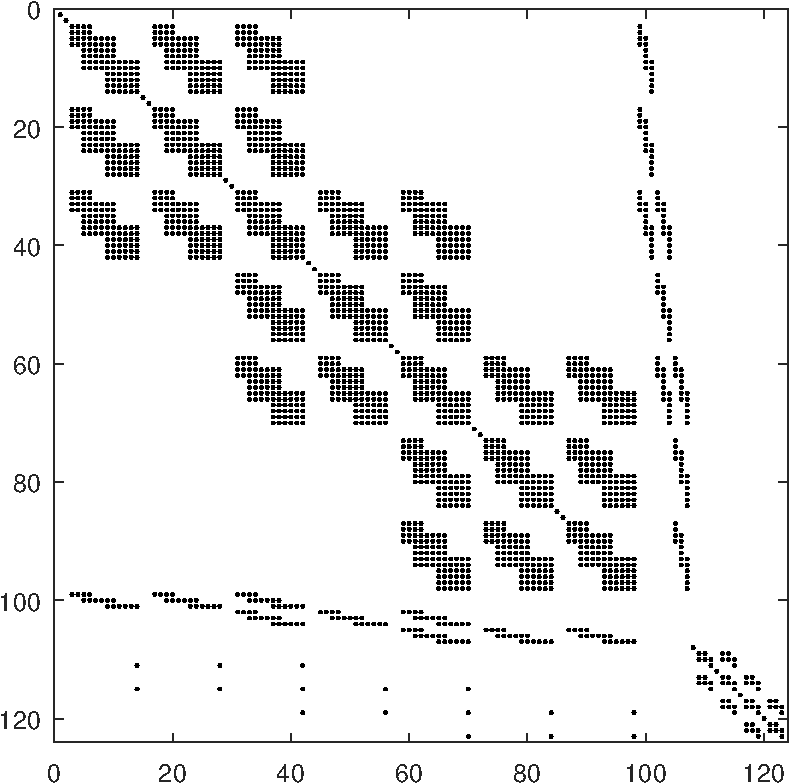
\includegraphics[width=0.5\textwidth]{figs/coarsespy.pdf}
\end{center}
\caption{FIXME block structure of coupled problem}
\label{fig:blockstructure}
\end{figure}

\section{Results}

FIXME among many things cite \cite{LeysingerGudmundsson2004} regarding earlier comparison of stokes to Halfar


\section{Discussion}

FIXME not appreciated that, while for explicit time-stepping schemes the surface mass balance need only be computed at the current ice surface, and at neighboring ice-free locations, in implicit time stepping the surface mass balance must be available to the evolving-geometry model (specifically to the residual-evaluation code) at every location in a 3D neighborhood of the ice surface, and indeed at all 3D locations above the bedrock elevation; a ``potential ice surface mass balance'' is needed at all such locations

\appendix
\section{Halfar solution to the shallow ice approximation}

In section FIXME, states of a certain similarity solution to an approximation of the Stokes problem are used as synthetic geometries for testing.  They arise from the $n=3$, isothermal, flat-bed ($b=0$), and zero surface mass balance ($a=0$) case of the shallow ice approximation (SIA).  This model, whose derivation is summarized in section \ref{sec:strongform}, determines an evolving ice thickness function $H(t,x,y)$ according to a nonlinear, free-boundary diffusion which applies on the set where $H>0$ \cite{Fowler1997}:
\begin{equation}
\frac{\partial H}{\partial t} = \Gamma \Div \left(H^5 |\grad H|^2 \grad H\right). \label{sia}
\end{equation}
(References \cite{Bueler2016,JouvetBueler2012} consider the rigorous meaning of this free boundary problem.)  In this equation we define $\Gamma = \frac{2}{5} A_3 (\rho g)^n$; constants $A_3,\rho,g$ have the same meaning and values as in the body of the paper.

P.~Halfar \cite{Halfar1981} observed that \eqref{sia} has an exact similarity solution with $\lim_{t\to 0} H$ equal to a multiple of the Dirac delta function, and that this solution is asymptotically stable.  In 3D \cite{Halfar1983} the solution is a circular dome which spreads radially while thinning, with constant-in-time total volume.  Denoting the usual radial coordinate as $r=(x^2+y^2)^{1/2}$, the solution is of the form $H(t,r) = t^{-\alpha} \varphi(s)$ with similarity variable $s=t^{-\beta} r$ and $\alpha=1/9$ and $\beta=1/18$.  If $H_0$ is a given central thickness value at a time $t_0$, and $R_0$ is a given radius, then the solution is
\begin{equation}
H(t,x,y) = H_0 \left(\frac{t}{t_0}\right)^{-\alpha} \left\{1 - \left[\left(\frac{t}{t_0}\right)^{-\beta} \frac{r}{R_0}\right]^{4/3}\right\}^{3/7}. \label{halfar}
\end{equation}
This formula applies where the resulting value is positive, and $H=0$ otherwise; see \cite{Bueleretal2005}.  The characteristic time can by found by $t_0 = (\beta/\Gamma) (7/4)^3 R_0^4 H_0^{-7}$.  The corresponding 2D Halfar solution $H(t,x)$ \cite{Halfar1981}, in one horizontal dimension, is of the same form as \eqref{halfar}, but with $r$ replaced by $x$ and with $\alpha=\beta=1/11$.

\small

\bigskip
\bibliography{simp}
\bibliographystyle{siam}

\end{document}
